\documentclass[letterpaper]{article}

\usepackage{tikz}
\usepackage{subcaption}
\usepackage{float}


\begin{document}
\section{Examples}

\subsection{Example 1: Mediator model ($ X \rightarrow M \rightarrow Y $):} All effects = $ 0.3 $. Left marginal correlation, right conditional

\begin{figure}[H]
	\centering
	\begin{subfigure}{0.5 \textwidth}
		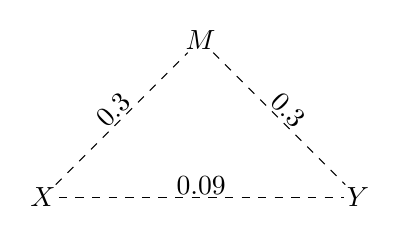
\begin{tikzpicture}[scale=2]
				\tikzstyle{every node}=[inner sep=1pt, align=center]
				\node (X) at (0, 0) {$ X $};
				\node (M) at (1, 1) {$ M $};
				\node (Y) at (2, 0) {$ Y $};
				\draw [dashed] (X) -- (M) node[midway, above, sloped] {$0.3$};
				\draw [dashed] (M) -- (Y) node[midway, above, sloped] {$0.3$};
				\draw [dashed] (X) -- (Y) node[midway, above, sloped] {$0.09$};
		\end{tikzpicture}
	\end{subfigure}%
	\begin{subfigure}{0.5 \textwidth}
		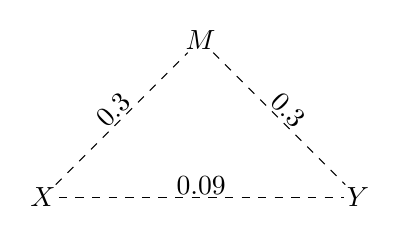
\begin{tikzpicture}[scale=2]
				\tikzstyle{every node}=[inner sep=1pt, align=center]
				\node (X) at (0, 0) {$ X $};
				\node (M) at (1, 1) {$ M $};
				\node (Y) at (2, 0) {$ Y $};
				\draw [dashed] (X) -- (M) node[midway, above, sloped] {$0.3$};
				\draw [dashed] (M) -- (Y) node[midway, above, sloped] {$0.3$};
				\draw [dashed] (X) -- (Y) node[midway, above, sloped] {$0.09$};
		\end{tikzpicture}
	\end{subfigure}
\end{figure}

Add edge $ M \rightarrow Y $:

\begin{figure}[H]
	\centering
	\begin{subfigure}{0.5 \textwidth}
		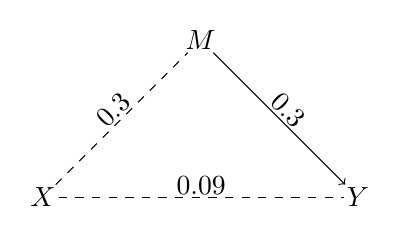
\begin{tikzpicture}[scale=2]
				\tikzstyle{every node}=[inner sep=1pt, align=center]
				\node (X) at (0, 0) {$ X $};
				\node (M) at (1, 1) {$ M $};
				\node (Y) at (2, 0) {$ Y $};
				\draw [dashed] (X) -- (M) node[midway, above, sloped] {$0.3$};
				\draw [->] (M) -- (Y) node[midway, above, sloped] {$0.3$};
				\draw [dashed] (X) -- (Y) node[midway, above, sloped] {$0.09$};
		\end{tikzpicture}
	\end{subfigure}%
	\begin{subfigure}{0.5 \textwidth}
		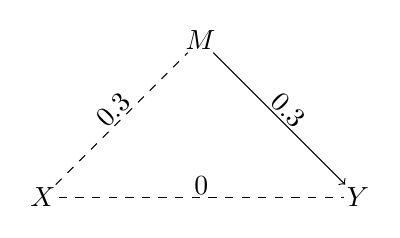
\begin{tikzpicture}[scale=2]
				\tikzstyle{every node}=[inner sep=1pt, align=center]
				\node (X) at (0, 0) {$ X $};
				\node (M) at (1, 1) {$ M $};
				\node (Y) at (2, 0) {$ Y $};
				\draw [dashed] (X) -- (M) node[midway, above, sloped] {$0.3$};
				\draw [->] (M) -- (Y) node[midway, above, sloped] {$0.3$};
				\draw [dashed] (X) -- (Y) node[midway, above, sloped] {$0$};
		\end{tikzpicture}
	\end{subfigure}
\end{figure}

Add edge $ X \rightarrow M $:

\begin{figure}[H]
	\centering
	\begin{subfigure}{0.5 \textwidth}
		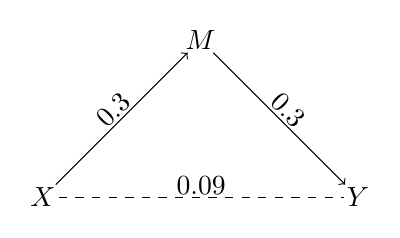
\begin{tikzpicture}[scale=2]
				\tikzstyle{every node}=[inner sep=1pt, align=center]
				\node (X) at (0, 0) {$ X $};
				\node (M) at (1, 1) {$ M $};
				\node (Y) at (2, 0) {$ Y $};
				\draw [->] (X) -- (M) node[midway, above, sloped] {$0.3$};
				\draw [->] (M) -- (Y) node[midway, above, sloped] {$0.3$};
				\draw [dashed] (X) -- (Y) node[midway, above, sloped] {$0.09$};
		\end{tikzpicture}
	\end{subfigure}%
	\begin{subfigure}{0.5 \textwidth}
		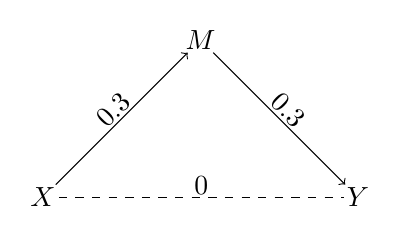
\begin{tikzpicture}[scale=2]
				\tikzstyle{every node}=[inner sep=1pt, align=center]
				\node (X) at (0, 0) {$ X $};
				\node (M) at (1, 1) {$ M $};
				\node (Y) at (2, 0) {$ Y $};
				\draw [->] (X) -- (M) node[midway, above, sloped] {$0.3$};
				\draw [->] (M) -- (Y) node[midway, above, sloped] {$0.3$};
				\draw [dashed] (X) -- (Y) node[midway, above, sloped] {$0$};
		\end{tikzpicture}
	\end{subfigure}
\end{figure}

Add edge $ X \rightarrow Y $ in the marginal case:

\begin{figure}[H]
	\begin{subfigure}{0.5 \textwidth}
		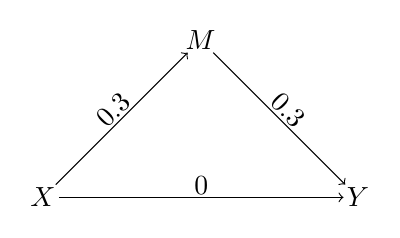
\begin{tikzpicture}[scale=2]
				\tikzstyle{every node}=[inner sep=1pt, align=center]
				\node (X) at (0, 0) {$ X $};
				\node (M) at (1, 1) {$ M $};
				\node (Y) at (2, 0) {$ Y $};
				\draw [->] (X) -- (M) node[midway, above, sloped] {$0.3$};
				\draw [->] (M) -- (Y) node[midway, above, sloped] {$0.3$};
				\draw [->] (X) -- (Y) node[midway, above, sloped] {$0$};
		\end{tikzpicture}
	\end{subfigure}
	\begin{subfigure}{0.5 \textwidth}
	\end{subfigure}
\end{figure}

\subsection{Example 2: Mediator with edge $ X \rightarrow Y $}

Add edge $ M \rightarrow Y $:

\begin{figure}[H]
	\centering
	\begin{subfigure}{0.5 \textwidth}
		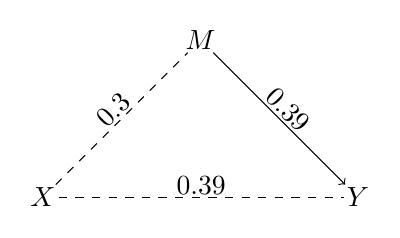
\begin{tikzpicture}[scale=2]
				\tikzstyle{every node}=[inner sep=1pt, align=center]
				\node (X) at (0, 0) {$ X $};
				\node (M) at (1, 1) {$ M $};
				\node (Y) at (2, 0) {$ Y $};
				\draw [dashed] (X) -- (M) node[midway, above, sloped] {$0.3$};
				\draw [->] (M) -- (Y) node[midway, above, sloped] {$0.39$};
				\draw [dashed] (X) -- (Y) node[midway, above, sloped] {$0.39$};
		\end{tikzpicture}
	\end{subfigure}%
	\begin{subfigure}{0.5 \textwidth}
		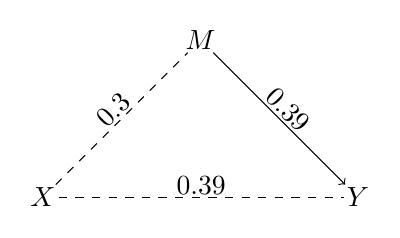
\begin{tikzpicture}[scale=2]
				\tikzstyle{every node}=[inner sep=1pt, align=center]
				\node (X) at (0, 0) {$ X $};
				\node (M) at (1, 1) {$ M $};
				\node (Y) at (2, 0) {$ Y $};
				\draw [dashed] (X) -- (M) node[midway, above, sloped] {$0.3$};
				\draw [->] (M) -- (Y) node[midway, above, sloped] {$0.39$};
				\draw [dashed] (X) -- (Y) node[midway, above, sloped] {$0.39$};
		\end{tikzpicture}
	\end{subfigure}
\end{figure}

Add edge $ X \rightarrow Y $:

\begin{figure}[H]
	\centering
	\begin{subfigure}{0.5 \textwidth}
		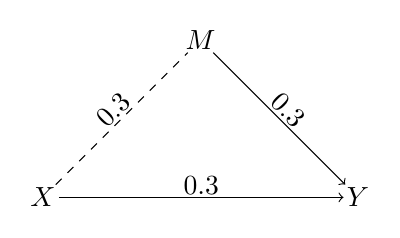
\begin{tikzpicture}[scale=2]
				\tikzstyle{every node}=[inner sep=1pt, align=center]
				\node (X) at (0, 0) {$ X $};
				\node (M) at (1, 1) {$ M $};
				\node (Y) at (2, 0) {$ Y $};
				\draw [dashed] (X) -- (M) node[midway, above, sloped] {$0.3$};
				\draw [->] (M) -- (Y) node[midway, above, sloped] {$0.3$};
				\draw [->] (X) -- (Y) node[midway, above, sloped] {$0.3$};
		\end{tikzpicture}
	\end{subfigure}%
	\begin{subfigure}{0.5 \textwidth}
		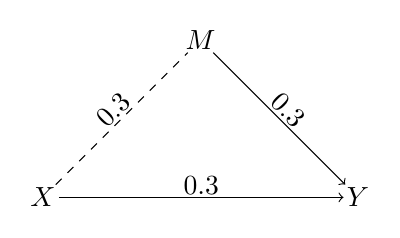
\begin{tikzpicture}[scale=2]
				\tikzstyle{every node}=[inner sep=1pt, align=center]
				\node (X) at (0, 0) {$ X $};
				\node (M) at (1, 1) {$ M $};
				\node (Y) at (2, 0) {$ Y $};
				\draw [dashed] (X) -- (M) node[midway, above, sloped] {$0.3$};
				\draw [->] (M) -- (Y) node[midway, above, sloped] {$0.3$};
				\draw [->] (X) -- (Y) node[midway, above, sloped] {$0.3$};
		\end{tikzpicture}
	\end{subfigure}
\end{figure}

Add edge $ X \rightarrow M $:

\begin{figure}[H]
	\centering
	\begin{subfigure}{0.5 \textwidth}
		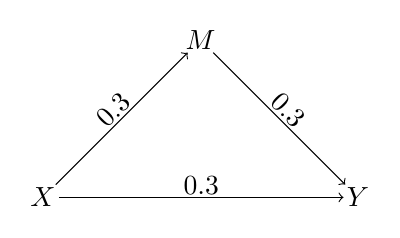
\begin{tikzpicture}[scale=2]
				\tikzstyle{every node}=[inner sep=1pt, align=center]
				\node (X) at (0, 0) {$ X $};
				\node (M) at (1, 1) {$ M $};
				\node (Y) at (2, 0) {$ Y $};
				\draw [->] (X) -- (M) node[midway, above, sloped] {$0.3$};
				\draw [->] (M) -- (Y) node[midway, above, sloped] {$0.3$};
				\draw [->] (X) -- (Y) node[midway, above, sloped] {$0.3$};
		\end{tikzpicture}
	\end{subfigure}%
	\begin{subfigure}{0.5 \textwidth}
		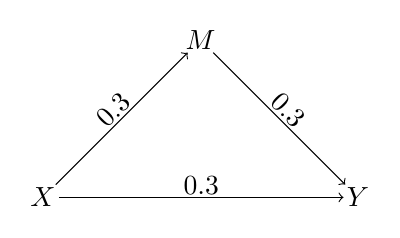
\begin{tikzpicture}[scale=2]
				\tikzstyle{every node}=[inner sep=1pt, align=center]
				\node (X) at (0, 0) {$ X $};
				\node (M) at (1, 1) {$ M $};
				\node (Y) at (2, 0) {$ Y $};
				\draw [->] (X) -- (M) node[midway, above, sloped] {$0.3$};
				\draw [->] (M) -- (Y) node[midway, above, sloped] {$0.3$};
				\draw [->] (X) -- (Y) node[midway, above, sloped] {$0.3$};
		\end{tikzpicture}
	\end{subfigure}
\end{figure}

\subsection{Example 3}
\begin{figure}[H]
	\begin{subfigure}{0.5 \textwidth}
		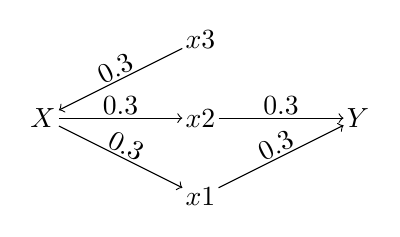
\begin{tikzpicture}[scale=2]
				\tikzstyle{every node}=[inner sep=1pt, align=center]
				\node (X) at (0, 0) {$ X $};
				\node (x1) at (1, -0.5) {$ x1 $};
				\node (x2) at (1, 0) {$ x2 $};
				\node (x3) at (1, 0.5) {$ x3 $};
				\node (Y) at (2, 0) {$ Y $};
				\draw [->] (x3) -- (X) node[midway, above, sloped] {$0.3$};
				\draw [->] (x1) -- (Y) node[midway, above, sloped] {$0.3$};
				\draw [->] (x2) -- (Y) node[midway, above, sloped] {$0.3$};
				\draw [->] (X) -- (x1) node[midway, above, sloped] {$0.3$};
				\draw [->] (X) -- (x2) node[midway, above, sloped] {$0.3$};
		\end{tikzpicture}
	\end{subfigure}%
	\begin{subfigure}{0.5 \textwidth}
	\end{subfigure}
	\caption{True Model}
\end{figure}

\begin{figure}[H]
	\begin{subfigure}{0.5 \textwidth}
		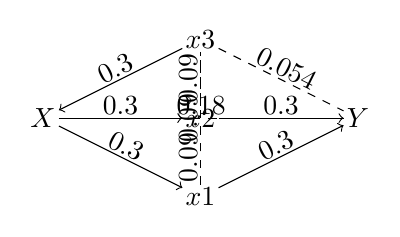
\begin{tikzpicture}[scale=2]
				\tikzstyle{every node}=[inner sep=1pt, align=center]
				\node (X) at (0, 0) {$ X $};
				\node (x1) at (1, -0.5) {$ x1 $};
				\node (x2) at (1, 0) {$ x2 $};
				\node (x3) at (1, 0.5) {$ x3 $};
				\node (Y) at (2, 0) {$ Y $};
				\draw [->] (x3) -- (X) node[midway, above, sloped] {$0.3$};
				\draw [->] (x1) -- (Y) node[midway, above, sloped] {$0.3$};
				\draw [->] (x2) -- (Y) node[midway, above, sloped] {$0.3$};
				\draw [->] (X) -- (x1) node[midway, above, sloped] {$0.3$};
				\draw [->] (X) -- (x2) node[midway, above, sloped] {$0.3$};
				\draw [dashed](X) -- (Y) node[midway, above, sloped] {$0.18$};
				\draw [dashed](x1) -- (x2) node[midway, above, sloped] {$0.09$};
				\draw [dashed](x1) -- (x3) node[midway, above, sloped] {$0.09$};
				\draw [dashed](x2) -- (x3) node[midway, above, sloped] {$0.09$};
				\draw [dashed](x3) -- (Y) node[midway, above, sloped] {$0.054$};
		\end{tikzpicture}
	\end{subfigure}%
	\begin{subfigure}{0.5 \textwidth}
		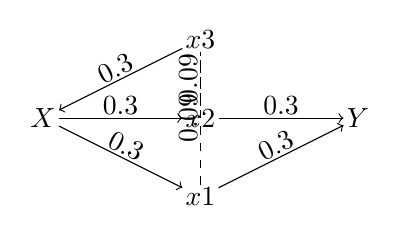
\begin{tikzpicture}[scale=2]
				\tikzstyle{every node}=[inner sep=1pt, align=center]
				\node (X) at (0, 0) {$ X $};
				\node (x1) at (1, -0.5) {$ x1 $};
				\node (x2) at (1, 0) {$ x2 $};
				\node (x3) at (1, 0.5) {$ x3 $};
				\node (Y) at (2, 0) {$ Y $};
				\draw [->] (x3) -- (X) node[midway, above, sloped] {$0.3$};
				\draw [->] (x1) -- (Y) node[midway, above, sloped] {$0.3$};
				\draw [->] (x2) -- (Y) node[midway, above, sloped] {$0.3$};
				\draw [->] (X) -- (x1) node[midway, above, sloped] {$0.3$};
				\draw [->] (X) -- (x2) node[midway, above, sloped] {$0.3$};
				\draw [dashed](x1) -- (x3) node[midway, above, sloped] {$0.09$};
				\draw [dashed](x2) -- (x3) node[midway, above, sloped] {$0.09$};
		\end{tikzpicture}
	\end{subfigure}
	\caption{(Left) Marginal (Right) Conditional}
\end{figure}


\section{Empirical Analysis}

Method:
\begin{enumerate}
	\item Start with a random DAG on $ 10 $ nodes.
	\item Simulate data from it, $ N = 500 $.
	\item Apply a threshold of $ 0.05 $ on correlations.
	\item Add edges for remaining correlations. Use an oracle for determining the direction. Based on the accuracy value, oracle either returns the true direction or randomly chooses the direction or don't know.
	\item If pruning, after each added edge remove any edge with coefficient = 0.
	\item Compare the Structural Hamming Distance between true and learned model.
\end{enumerate}

\begin{figure}[H]
	\begin{subfigure}{0.5 \textwidth}
		\centering
		\includegraphics{../code/plots/shd.pdf}
	\end{subfigure}%
	\begin{subfigure}{0.5 \textwidth}
		\centering
		\includegraphics{../code/plots/shd_pruned.pdf}
	\end{subfigure}
		\caption{Mean SHD with varying edge probabilities and oracle accuracy (Left) Without Pruning (Right) With pruning. Compared to Hill-Climb Search with BIC score}
\end{figure}

Remarks:
\begin{enumerate}
	\item After drawing an edge, the parameter values can change.
	\item Pruning is needed in both marginal and conditional cases.
	\item In the marginal case, the ``suggested'' graph is more dense.
	\item Results with pruning vs non pruning seems close. Unexpected, need to check for bugs in the code.
\end{enumerate}

\end{document}
